\section{Begrifflichkeiten}
In der Praxis sind viele, in dieser Arbeit häufig verwendete, Begriffe unterschiedlich belegt. Aus diesem Grund soll im Folgenden eindeutig klargestellt werden, was mit den verwendeten Begriffen tatsächlich gemeint ist.

\begin{description}
	\item [App (plural: Apps)]
		In dieser Arbeit werden Programme die speziell für Smartphones entwickelt wurden als Apps bezeichnet. Implizit wird hiermit auch die Plattform auf Android oder iOS eingrenzt. Der Begriff App zeichnet sich in dieser Arbeit dadurch aus, dass die damit gemeinte Anwendung für den Nutzer sehr einfach zu installieren ist. In der Regel beziehen Nutzer Apps aus einem Shop des Hersteller beispielsweise Apples AppStore und starten diese über ein Icon auf dem Startbildschirm des Betriebssystems.
		
	\item [Webseite, Webanwendung und Web App]
		Der Begriff Webseite wird in dieser Arbeit für HTML-basierte Inhalte verwendet, die der*die Nutzer*in über den Browser abruft.
		
		Die Webanwendung unterscheidet sich dahingehen, dass sie dynamisch auf den Nutzer reagiert und seine Eingaben auswertet und gegebenenfalls den angezeigten Inhalt ändert oder nachlädt. Speziell werden JavaScript basierte Anwendungen in dieser Arbeit als Webanwendung oder Web App bezeichnet. Web App und Webanwendung werden synonym verwendet.
		
		Eine Webseite kann, aber muss keine Webanwendung oder Web App sein.
	
	\item [Progressive Web App]
		Eine Progressive Web App ist eine Webseite und speziell eine Webanwendung oder Web App, welche dynamisch auf den Nutzer reagiert.
		In dieser Arbeit werden Webanwendungen, welche lokal auf einem Gerät installiert werden können als \acf{pwa} bezeichnet. Die PWA kann als Webanwendung oder Web App bezeichnet werden, welche die Kriterien aus Kapitel \ref{chap:pwa} erfüllt.
		
		Im Unterschied zur nativen App kann die selbe PWA sowohl auf Smartphones, als auch auf eine Desktopgerät (Notebook, Desktop Computer etc.) installiert werden.
		
	\item [Desktop PWA]
		Mit Desktop PWA ist hier explizit eine Progressive Web App gemeint, welche auf einem Desktopgerät installiert wird.
			
	\item [native App]
		Diese Arbeit beschäftigt sich mit einer modernen Methode Mobilanwendungen zu programmieren: der PWA. Im Unterschied dazu ist eine native App in Java oder Swift geschrieben und ist damit stark plattformabhängig. Nativ implementiere Apps sind entweder für iOS oder Android entwickelt worden, nicht aber für mehrere Plattformen.
	
\end{description}

\section{Progressive Web App}
\label{chap:pwa}

%\subsection{Charakteristiken einer \ac{pwa}}
Zu Beginn dieses Unterkapitels soll die bereits erwähnte \acf{pwa} erklärt werden. Anschließend folgen die verwendeten Frameworks für die Entwicklung der PWA. Ein Überblick über diese ist essenziell für das Verständnis von Kapitel \ref{chap:implementierung}, in welchem die Implementierungsschritte betrachtet werden.

Eine Progressive Web App ist ein nächster Schritt nach der Dynamisierung statischer HTML-Seiten durch JavaScript und Frontendframeworks. Der Software Entwickler und Author Majid Hajian charakterisiert PWAs mit acht Eigenschaften. Die wichtigsten dieser Charakteristika werden im Folgenden zusammenfassend erläutert:


\begin{description}
  \item [Installierbarkeit]
	  Der*die Nutzer*in einer Webanwendung kann diese lokal auf seinem Gerät installieren. Sie kann anschließend, wie eine native App, vom Startbildschirm gestartet werden. Um die Webanwendung zu Nutzen muss ein*e Nutzer*in keinen Zwischenschritt mehr über den Browser tätigen.
  
  \item [Ähnlichkeit mit einer nativ implementierten App]  
 	 Klassischerweise werden Android-Apps in Java und iOS Apps in Swift programmiert. Die PWA soll, wie eine native App, auf die Hardware des Mobilgeräts zugreifen können (beispielsweise die Nutzung Bluetooth-Chips). Außerdem unterscheidet sich das User Interface der PWA nicht maßgeblich von der nativen App. 
  
  \item [Offline-Verwendung] 
  	Die PWA soll unabhängig von Netzwerkverbindung funktionieren. Sie ist nach dem "offline-first-design" konzipiert. Die Google-Chrome Dokumentation für Cloud-Entwickler beschreibt Offline First Apps als Webanwendung, deren Dateien (JavaScript, HTML, CSS etc.) bereits heruntergeladen sind. Daten werden temporär über eine Browser-Schnittstelle gespeichert und bei Bedarf synchronisiert. Außerdem kann die Anwendung auf eine unterbrochene Netzwerkverbindungen reagieren \cite{GoogleOfflineApps}. Die PWA ist demnach eine Webanwendung, die sowohl online, als auch offline nutzbar ist.

  \item [Mobiloptimiert]  
  	Die PWA ist für die (meist leistungsschwache) Mobilhardware konzipiert und funktioniert hierauf ohne Performanceprobleme. Hajian legt besonders auf das schnelle Laden beim Start der Anwendung wert.
  	
  \item [Informierung des*der Nutzers*in] 
  	Wie native Apps, kann die PWA den Nutzer über Push-Nachrichten informieren oder zu Interaktion auffordern.
\end{description}

\cite[S. 1f.]{Hajian2019}
Diese Charakteristiken decken sich mit der Beschreibung durch die Entwickler-Dokumentation der PWA von Google. Im Vergleich zu Hijian ist diese etwas spezifischer und erwähnt beispielsweise die Kontrolle des Anwendungscaches durch einen JavaScript Service Worker (siehe Kapitel \ref{chap:service_worker}), um die Abhängikeit von einer Netzwerkverbindung aufzuheben.
\cite{GooglePWAOverview}

\subsection{Installation einer PWA}

Diese Arbeit betrachtet die PWA, da sie (wie eine native Anwendung) lokal auf einem Gerät installiert werden kann. Es ist dafür kein zentraler Shop nötig: die Installation wird über den Browser gestartet.

\begin{figure}[h]
        \centering
        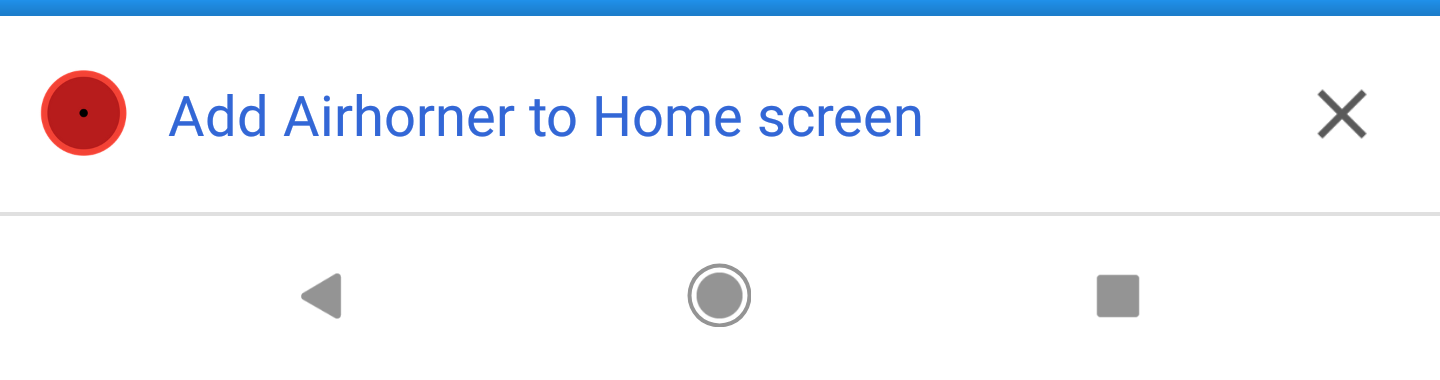
\includegraphics[scale=0.2]{img/a2hs-infobar-cropped.png}
        \caption{Browserdialog zur Installation einer PWA \cite{PWAAddToHomeScreenPrompt}}
        \label{fig:pwainstallationprompt}
\end{figure}

Die Aufforderung zur Installation einer PWA kann entweder über den Browser (siehe Abbildung \ref{fig:pwainstallationprompt}) erfolgen oder über ein Element der Website, dass ein Event erzeugt, wie beispielsweise ein Button oder ein Dialog. 

Zwar bezeichnen Browser die Installation meist nur als \texttt{Zum Startbildschirm hinzufügen} tatsächlich generiert der Browser aber dann eine WebAPK, welche auf dem Gerät installiert wird. Auf Desktopgeräte startet die PWA in einem eignen stark verschlankten Browserfenster ohne Suchleiste und Bedienelemente. \cite{GooglePWAInstallation}


\subsection{Manifest Datei}

Um die PWA auf einem Gerät installieren zu können, muss es eine web-app-manifest Datei zur Verfügung gestellt werden. Diese ist ein JSON file, welche als Konfigurationsdatei der installierten Anwendung dient. \cite{GooglePWAManifest}

\begin{listing}[H]
    \inputminted{json}{sourcecode/manifest_sample.json}
    \caption{Manifestdatei einer PWA}
      \label{sourcecode:manifest_sample}
\end{listing}

%\begin{figure}[h]
%%        \centering
 %       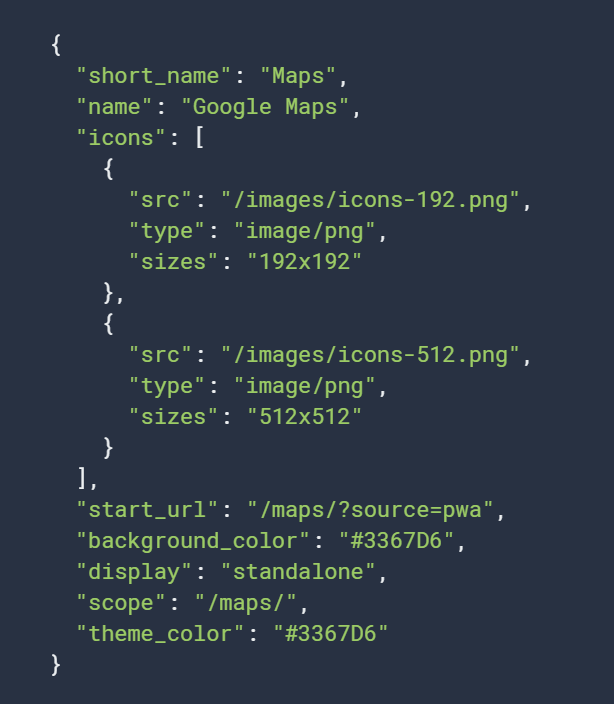
\includegraphics[scale=0.6]{img/sample_manifest.png}
 %       \caption{Manifestdatei einer PWA}
 %       \label{fig:manifest_sample}
        %https://developers.google.com/web/fundamentals/web-app-manifest?hl=en
%\end{figure}

Abbildung \ref{sourcecode:manifest_sample} zeigt den Inhalt einer Manifest-Datei. Neben diversen Icons (Zeile 4-15) werden auch \textbf{Name} (Zeile 3), \textbf{Farbschema} (Zeile 20) und \textbf{Anzeigeeinstellungen} (Zeile 18) festgelegt.
Die Manifest-Datei wird im HTML der Webanwendung eingebunden, siehe Abbildung \ref{sourcecode:manifest_include}. 

Es ist die Einfachheit dieses Prozesses hervorzuheben: Das Hinzufügen einer (wenige Zeilen langer) JSON-Datei macht die gesamte Webanwendung installierbar. Es wird kein App-Store, manueller Dateidownload oder Installer benötigt. 

\begin{listing}[H]
    \inputminted{xml}{sourcecode/include_manifest.html}
    \caption{Einbinden der Manifestdatei}
      \label{sourcecode:manifest_include}
              %https://developers.google.com/web/fundamentals/web-app-manifest?hl=en
\end{listing}

%\begin{figure}[h]
%        \centering
%%        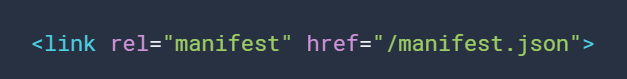
\includegraphics[scale=0.7]{img/include_manifest.png}
 %%       \caption{Einfache Einbindung des Manifests}
  %      \label{sourcecode:manifest_include}
        %https://developers.google.com/web/fundamentals/web-app-manifest?hl=en
%\end{figure}


\subsection{Service Worker}
\label{chap:service_worker}

Damit die PWA trotz fehlender Netzwerkverbindung funktioniert wird ein besonderer Mechanismus benötigt: der Service Worker. Mit ihm können Abhängigkeiten der App lokal gecached werden, so dass die Anwendung auch bei schlechter oder gar fehlender Netzwerkverbindung funktioniert. \cite[S. 7]{BeginningPWA}

Ein Service Worker ist ein von der UI seperiertat laufendes Hintergrundscript der Webanwendung, siehe Abbildung \ref{fig:serviceWorker}. Er wird genutzt um Bilder, Scripte, Styles oder ganze Seiten zu cachen. Bei bestehender Netzwerkverbindung führt er nötige Synchronisierungen durch. Nicht zuletzt ist er auch für das senden von Push-Notifications zuständig. \cite[S. 24]{BeginningPWA}

\begin{figure}[h]
        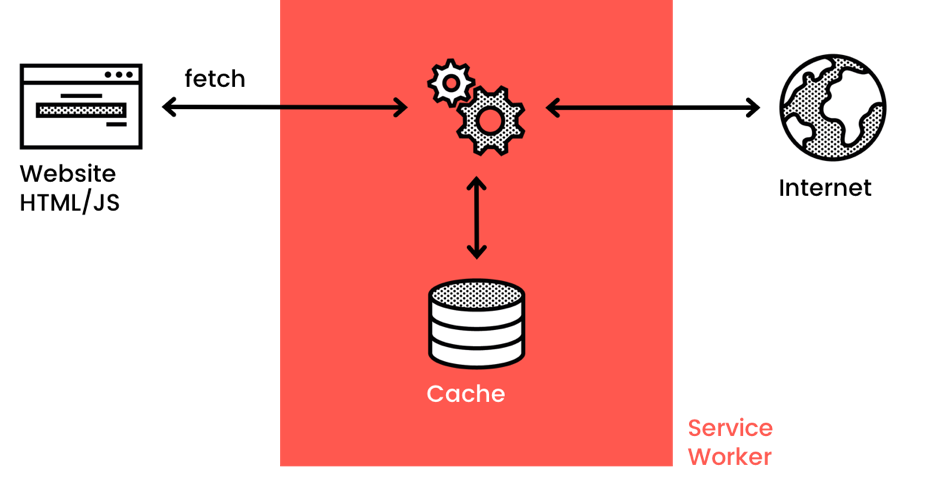
\includegraphics[width=\linewidth]{img/ServiceWorker-8a0968f1b295f1ff.png}
        \centering
        \caption{Konzept des Service Workers \cite{ServiceWorkerDiagramm}}
        \label{fig:serviceWorker}
\end{figure}


Alle verbreiteten Desktopbrowser wie Chrome, Firefox, Opera, Edge und mitterweile auch Safari unsterstützen das Service Worker Konzept. Der Mobile Chromebrowser unter Android unterstützt Service Worker bereits voll, während Safari unter iOS noch an diesem Feature arbeitet. \cite[S. 9]{BeginningPWA}


\subsection{Unterstütze Plattformen von PWA}
Das Projekt \textit{CanIUse} aggregiert Daten zu Webstandards des w3 Konsortiums und Browserdokumentationen. Es wird als Quelle für die Unterstützung von Features durch aktuelle Browser herangezogen.

Apples mobiler Browser Safari unterstützt eines der wichtigsten Features der PWA noch nicht vollständig: das Web App Manifest. Allerdings wird der Service Worker vollständig unterstützt \cite{CanIUseWebManifest}. Wann und ob Safari die Unterstützung für das Manifest implementiert ist unklar und bleibt abzuwarten. Die aktuelle Teilunterstützung zeigt jedoch, dass sich Apple nicht grundsätzlich gegen die PWA weigert.

 %Die Versionen zeigen aber eine stetig voranschreitende Integration der, erweitert den Funktionsumfang in den neusten Versionen von iOS. 

% https://medium.com/@firt/progressive-web-apps-on-ios-are-here-d00430dee3a7



% Source: https://developers.google.com/web/progressive-web-apps/desktop
Die Nutzung von PWAs ist nicht ausschließlich auf Smartphones begrenzt. Wie normale Desktopprogramme werden Desktop PWAs in einem eigenen Fenster gestartet. 
Der Unterschied zwischen den Bedienelementen nativer Desktopanwendungen und Desktop PWAs ist ausschließlich farblicher Natur. Stark vereinfacht beschrieben, sind Desktop PWAs Browserfenster ohne Tabs und Adressleiste. Durch die Nutzung von Service Workern, welche die Webanwendung cachen, sind auch Desktop PWAs nicht an eine Netzwerkverbindung gebunden.

Grundsätzlich können Desktop PWAs auf jedem Betriebssystem installiert werden, auf dem Google Chrome (Version größer 73) installiert werden kann: Windows, Mac, Linux und Chrome OS.
\cite{GooglePWADesktop}



\subsection{Node.js}

%NodeJSWebsiteAbout
Node.js ist eine open-source JavaScript Laufzeitumgebung für die Entwicklung skalierbarer Webanwendungen 
\cite{NodeJSWebsiteAbout}.
Selbst baut Node.js auf der V8-Engine auf, einer Laufzeitumgebung, die auch von Google Chrome genutzt wird 
%NodeJSRecepies
\cite[S. 1]{NodeJSRecepies}.
% PracitalNodeJS
Wegen zeitsparenden Features, wie automatischem Typecasting oder der Tatsache, dass Node.js alle Daten als Objekt behandelt, erfreut sich Node.js großer Beliebtheit 
\cite[S. 12]{PracitalNodeJS}.
Die Kombination mit dem Package Manager npm ermöglicht die einfache Installation und Nutzung von Modulen, um die Funktionalität der Plattform zu erweitern. 
\cite[S. 9]{NodeJSRecepies}.


\subsection{Angular}

Angular ist ein open-source Type-Script basiertes Framework zur Entwicklung von Webanwendungen, welches Node.js nutzt.


%https://octoverse.github.com/projects
Mit über Achttausend Mitwirkenden Entwicklern (Angular CLI) beziehungsweise über Siebentausend Mitwirkender (Angular Framework) belegt das Angular Command Line Interface und das Angular Framework die Plätze 4 und 6 der größten Projekte auf Github. 
% https://octoverse.github.com/projects
\cite{OctoverseGitHubStatistics}

Das Framework arbeitet auf Basis von Komponenten. Ein Eingabefeld, Seite oder eine Liste werden in Angular als solche Komponenten seperat betrachtet. Auch in der Dateistruktur werden Komponenten stark getrennt. Jede Komponente besitzt beispielsweise ein eigenes CSS (oder SCSS) und HTML-File. Eine Komponente für eine Seite kann so auch eine oder sogar mehrere Listenkomponenten einbinden. Durch die Wiederverwendung von Code-Fragmenten in Komponenten wird der Programmcode sehr übersichtlich und strukturiert.

\begin{figure}[h]
        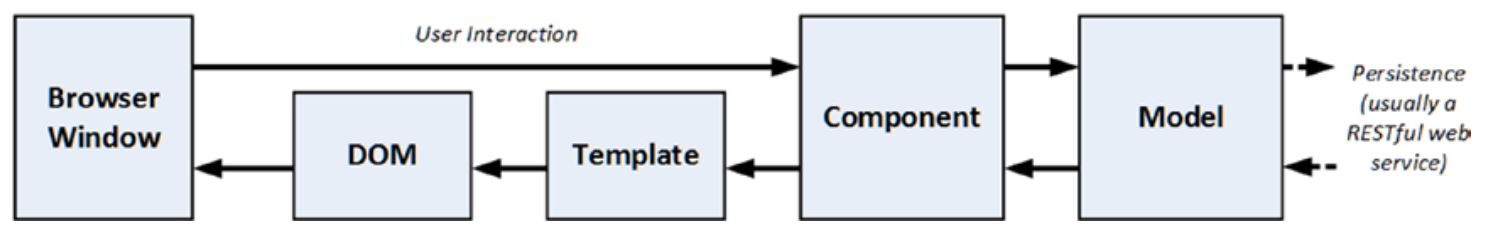
\includegraphics[width=\linewidth]{img/Angular_MVC.JPG}
        \centering
        \caption{MVC Konzept von Angular \cite[S. 35, Abbildung 3-4]{ProAngular}}
        \label{fig:angularmvc}
\end{figure}

Eine Angular Anwendung ist in drei Einheiten gegliedert:\\

\textbf{Model}\\ 
Enthält Logik für die Verwaltung von Daten, beispielsweise das Erstellen, Speichern oder Modifizieren. Dies kann über die Kommunikation mit einem Webserve via REST-API erfolgen. Das Model enhält keine Logik, um mit dem Nutzer zu interagieren.\\

\textbf{Component}\\
Enthält Logik für das Aktualisieren der Daten im Model aufgrund Nutzerinteraktion. \\

\textbf{Template}\\ 
Enthält Logik und Markup, um dem Nutzer Daten anzeigen zu können.

\cite{ProAngular}

\section{native Apps}

\subsection{iOS}

\subsection{Android}

\textbf{Entwicklung}

%Android apps are written in Java and use various Java application program interfaces (APIs).
%Because you’ll want to write your own apps, but may be unfamiliar with the Java language and these
%APIs, this book teaches you about Java as a first step into Android app development. It provides you
%with Java language fundamentals and Java APIs that are useful when developing apps.

Native Android Anwendungen werden in der Regel in Java entwickelt. Durch die Nutzung der zahlreichen APIs wird aus einem Java Programm eine native Android App.
\cite[S. 1]{JavaForAndroid}
Mittlerweile wird die teilweise veraltete Java-Syntax graduell durch die modernere Programmiersprache Kotlin abgelöst.
\cite{KotlinAndroid}


%Kotlin is a free and open source project under the Apache 2.0 license
%https://developer.android.com/kotlin

%https://kotlinlang.org/docs/reference/android-overview.html

Meist werden Android Apps mithilfe der Entwicklungsumgebung Android Studio entwickelt, welches auf der IntelliJ IDE von JetBrains aufbaut, aber von Google weiterentwickelt wird. Die IDE bietet Entwicklern unter anderem einen visuellen Layout Editor und eine Vielzahl von Android Emulatoren zum Testen der Apps auf verschiedenen Android Versionen und unterschiedlicher Hardware. Dafür wird jedoch performante Hardware zum Entwickeln benötigt: 8 Gigabyte Arbeitsspeicher oder mehr ist die Empfehlung der Herausgeber. \cite{AndroidStudio}

\textbf{Vertrieb}

Die meisten Apps beziehen Nutzer über den Google Play Store, einem Onlineshop für kostenlose und kostenpflichtige Android Anwendungen. 
Updates werden ebenfalls über den Play Store installiert. Alternativ kann ein Nutzer eine App in Form einer \texttt{.apk}-Datei installieren. Dieser Weg bleibt jedoch aufgrund der Umständlichkeit und unbekannten Sicherheitsprüfung der App weitestgehend ungenutzt.

\subsection{Grundlegendes}


\subsection{Installation einer nativen App}
\textbf{Android}\\